\documentclass{beamer}

\usepackage{listings}
\usepackage[T1]{fontenc}
\usepackage{lmodern}
\usepackage[utf8]{inputenc}
% Copyright 2017 Sergei Tikhomirov, MIT License
% https://github.com/s-tikhomirov/solidity-latex-highlighting/

\usepackage{listings, xcolor}

\definecolor{verylightgray}{rgb}{.97,.97,.97}

\lstdefinelanguage{Solidity}{
	keywords=[1]{anonymous, assembly, assert, balance, break, call, callcode, case, catch, class, constant, continue, constructor, contract, debugger, default, delegatecall, delete, do, else, emit, event, experimental, export, external, false, finally, for, function, gas, if, implements, import, in, indexed, instanceof, interface, internal, is, length, library, log0, log1, log2, log3, log4, memory, modifier, new, payable, pragma, private, protected, public, pure, push, require, return, returns, revert, selfdestruct, send, solidity, storage, struct, suicide, super, switch, then, this, throw, transfer, true, try, typeof, using, value, view, while, with, addmod, ecrecover, keccak256, mulmod, ripemd160, sha256, sha3}, % generic keywords including crypto operations
	keywordstyle=[1]\color{blue}\bfseries,
	keywords=[2]{address, bool, byte, bytes, bytes1, bytes2, bytes3, bytes4, bytes5, bytes6, bytes7, bytes8, bytes9, bytes10, bytes11, bytes12, bytes13, bytes14, bytes15, bytes16, bytes17, bytes18, bytes19, bytes20, bytes21, bytes22, bytes23, bytes24, bytes25, bytes26, bytes27, bytes28, bytes29, bytes30, bytes31, bytes32, enum, int, int8, int16, int24, int32, int40, int48, int56, int64, int72, int80, int88, int96, int104, int112, int120, int128, int136, int144, int152, int160, int168, int176, int184, int192, int200, int208, int216, int224, int232, int240, int248, int256, mapping, string, uint, uint8, uint16, uint24, uint32, uint40, uint48, uint56, uint64, uint72, uint80, uint88, uint96, uint104, uint112, uint120, uint128, uint136, uint144, uint152, uint160, uint168, uint176, uint184, uint192, uint200, uint208, uint216, uint224, uint232, uint240, uint248, uint256, var, void, ether, finney, szabo, wei, days, hours, minutes, seconds, weeks, years},	% types; money and time units
	keywordstyle=[2]\color{teal}\bfseries,
	keywords=[3]{block, blockhash, coinbase, difficulty, gaslimit, number, timestamp, msg, data, gas, sender, sig, value, now, tx, gasprice, origin},	% environment variables
	keywordstyle=[3]\color{violet}\bfseries,
	identifierstyle=\color{black},
	sensitive=false,
	comment=[l]{//},
	morecomment=[s]{/*}{*/},
	commentstyle=\color{gray}\ttfamily,
	stringstyle=\color{red}\ttfamily,
	morestring=[b]',
	morestring=[b]"
}

\lstset{
  language=Solidity,
  escapeinside={<@}{@>},
	backgroundcolor=\color{verylightgray},
	extendedchars=true,
	basicstyle=\footnotesize\ttfamily,
	showstringspaces=false,
	showspaces=false,
	numbers=left,
	numberstyle=\footnotesize,
	numbersep=9pt,
	tabsize=2,
	breaklines=true,
	showtabs=false,
	captionpos=b
}


\usecolortheme{beaver}
\addtobeamertemplate{footnote}{}{\vspace{4ex}}
\setbeamerfont{footnote}{size=\scriptsize}

\newcommand\blfootnote[1]{%
  \begingroup
  \renewcommand\thefootnote{}\footnote{#1}%
  \addtocounter{footnote}{-1}%
  \endgroup
}

\AtBeginSection
{
  \begin{frame}
    \frametitle{Table of Contents}
    \tableofcontents[currentsection]
  \end{frame}
}

\setbeamertemplate{itemize items}{\textbullet}
\setbeamertemplate{footline}[text line]{%
  \parbox{\linewidth}{\vspace*{-8pt}
    \insertshorttitle\hfill\insertshortauthor\hfill\insertframenumber
  }
}
\setbeamertemplate{navigation symbols}{}

\begin{document}

\title{Experiments in Formal Verification of Scala Code}
% \subtitle{The Decentralized Autonomous Organization}
\author{Ramon Boss, Anna Doukmak}

\date{2019-06-14}

\frame{\titlepage}


\begin{frame}
  \frametitle{Table of Contents}
  \tableofcontents
\end{frame}


%%%%%%%%%%%%%%%%%%%%%%%%%%%%%%%%%%%%%%%%%%%%%%%%%%%%%%%%%%%%%%%%%%%%%%%%%%%%%%%%
\section{Formal Verification}
%%%%%%%%%%%%%%%%%%%%%%%%%%%%%%%%%%%%%%%%%%%%%%%%%%%%%%%%%%%%%%%%%%%%%%%%%%%%%%%%


\begin{frame}
\frametitle{Stainless}
\begin{itemize}
  \item Pure Scala
  \item Pre- and Postcondition
  \item Outcome: valid, invalid, unknown
\end{itemize}
\end{frame}


\begin{frame}[fragile]
\frametitle{Example: max}
\begin{lstlisting}[language=Scala]
def max(x: Int, y: Int): Int = {
  val d = x - y
  if (d > 0) x
  else y
}
\end{lstlisting}
\blfootnote{\url{https://epfl-lara.github.io/stainless/tutorial.html\#warm-up-max}}
\end{frame}


\begin{frame}[fragile]
\frametitle{Example: max}
\begin{lstlisting}[language=Scala]
def max(x: Int, y: Int): Int = {
  val d = x - y
  if (d > 0) x
  else y
} ensuring (res =>
  x <= res && y <= res && (res == x || res == y))
\end{lstlisting}
\blfootnote{\url{https://epfl-lara.github.io/stainless/tutorial.html\#warm-up-max}}
\end{frame}


\begin{frame}[fragile]
\frametitle{Example: max}
{\small\begin{verbatim}
  [...     ]
  [  Info  ]  - Result for 'postcondition' VC for max @2:3:
  [Warning ]  => INVALID
  [Warning ] Found counter-example:
  [Warning ]   x: Int -> -2147483648
  [Warning ]   y: Int -> 2147483647
  [...     ]
\end{verbatim}}
% \begin{verbatim}
%   [Warning ] The Z3 native interface is not available. Falling back onto smt-z3.
% [  Info  ]  - Checking cache: 'postcondition' VC for max @2:3...
% [  Info  ]  - Checking cache: 'postcondition' VC for max @2:3...
% [  Info  ] Cache miss: 'postcondition' VC for max @2:3...
% [  Info  ] Cache miss: 'postcondition' VC for max @2:3...
% [  Info  ]  - Now solving 'postcondition' VC for max @2:3...
% [  Info  ]  - Now solving 'postcondition' VC for max @2:3...
% [  Info  ]  - Result for 'postcondition' VC for max @2:3:
% [Warning ]  => INVALID
% [Warning ] Found counter-example:
% [Warning ]   x: Int -> 1
% [Warning ]   y: Int -> -2147483648
% [  Info  ]  - Result for 'postcondition' VC for max @2:3:
% [Warning ]  => INVALID
% [Warning ] Found counter-example:
% [Warning ]   x: Int -> -2147483648
% [Warning ]   y: Int -> 2147483647
% [  Info  ]   ┌───────────────────┐
% [  Info  ] ╔═╡ stainless summary ╞══════════════════════════════════════════════════════════════════════╗
% [  Info  ] ║ └───────────────────┘                                                                      ║
% [  Info  ] ║ max    postcondition          invalid      U:smt-z3       Test.scala:2:3          0.908    ║
% [  Info  ] ║ max    postcondition          invalid      U:smt-z3       Test.scala:2:3          0.906    ║
% [  Info  ] ╟┄┄┄┄┄┄┄┄┄┄┄┄┄┄┄┄┄┄┄┄┄┄┄┄┄┄┄┄┄┄┄┄┄┄┄┄┄┄┄┄┄┄┄┄┄┄┄┄┄┄┄┄┄┄┄┄┄┄┄┄┄┄┄┄┄┄┄┄┄┄┄┄┄┄┄┄┄┄┄┄┄┄┄┄┄┄┄┄┄┄┄┄╢
% [  Info  ] ║ total: 2    valid: 0    (0 from cache) invalid: 2    unknown: 0    time:   1.814           ║
% [  Info  ] ╚════════════════════════════════════════════════════════════════════════════════════════════╝
% [  Info  ] Shutting down executor service.

% \end{verbatim}
\end{frame}

\begin{frame}[fragile]
  \frametitle{Example: max}
  \begin{lstlisting}[language=Scala]
  def max(x: Int, y: Int): Int = {
    require(0 <= x && 0 <= y)
    val d = x - y
    if (d > 0) x
    else y
  } ensuring (res =>
    x <= res && y <= res && (res == x || res == y))
  \end{lstlisting}
  \blfootnote{\url{https://epfl-lara.github.io/stainless/tutorial.html\#warm-up-max}}
  \end{frame}
  

\begin{frame}
\frametitle{Properties}
\begin{itemize}
  \item Bitcoin-S
  \item No-Inflation Property
  \item Addition-with-Zero Property
\end{itemize}
\end{frame}


%%%%%%%%%%%%%%%%%%%%%%%%%%%%%%%%%%%%%%%%%%%%%%%%%%%%%%%%%%%%%%%%%%%%%%%%%%%%%%%%
\section{Problems Verifying Bitcoin-S}
%%%%%%%%%%%%%%%%%%%%%%%%%%%%%%%%%%%%%%%%%%%%%%%%%%%%%%%%%%%%%%%%%%%%%%%%%%%%%%%%


\begin{frame}[fragile]
\frametitle{Turning Object into Case Object}
This:
\begin{lstlisting}[language=Scala]
object Satoshis extends BaseNumbers[Satoshis] {
  val zero = Satoshis(Int64.zero)
  val one = Satoshis(Int64.one)
}
\end{lstlisting}

Becomes this:
\begin{lstlisting}[language=Scala]
case object Satoshis extends BaseNumbers[Satoshis] {
  val zero = Satoshis(Int64.zero)
  val one = Satoshis(Int64.one)
}
\end{lstlisting}
\end{frame}


\begin{frame}[fragile]
\frametitle{Getting Rid of Abstract Type Member}
This:
\begin{lstlisting}[language=Scala]
sealed abstract class CurrencyUnit {
  type A

  protected def underlying: A
}

sealed abstract class Satoshis extends CurrencyUnit {
  override type A = Int64
}
\end{lstlisting}

Becomes this:
\begin{lstlisting}[language=Scala]
sealed abstract class CurrencyUnit {
  protected def underlying: Int64
}

sealed abstract class Satoshis extends CurrencyUnit
\end{lstlisting}
\end{frame}


\begin{frame}[fragile]
\frametitle{BigInt \&-Function to Bound Check}
This:
\begin{lstlisting}[language=Scala]
sealed abstract class Number {
  def andMask: BigInt
  def checkResult(result: BigInt): BigInt = {
    require((result & andMask) == result)
    result
  }
}  
\end{lstlisting}
Becomes this:
\begin{lstlisting}[language=Scala]
sealed abstract class Number {
  def checkResult(result: BigInt): BigInt = {
    require(
      result <= BigInt("9223372036854775807") &&
      result >= BigInt("-9223372036854775808")
    )
    result
  }
}
\end{lstlisting}
\end{frame}


\begin{frame}[fragile]
\frametitle{Formal Specification}
\begin{lstlisting}[language=Scala]
def +(c: CurrencyUnit): CurrencyUnit = {
  require(c.satoshis == Satoshis.zero)
  Satoshis(
    satoshis.underlying + c.satoshis.underlying
  )
} ensuring(res => res.satoshis == this.satoshis)
\end{lstlisting}
\end{frame}


\begin{frame}
\frametitle{Output of Stainless}
\centering
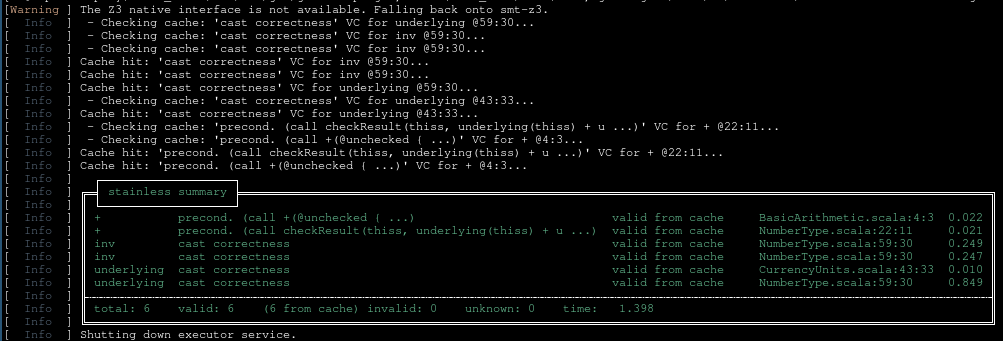
\includegraphics[width=\textwidth,height=0.8\textheight,keepaspectratio]{assets/final_verify_output.png}
\end{frame}


%%%%%%%%%%%%%%%%%%%%%%%%%%%%%%%%%%%%%%%%%%%%%%%%%%%%%%%%%%%%%%%%%%%%%%%%%%%%%%%%
\section{Conclusion}
%%%%%%%%%%%%%%%%%%%%%%%%%%%%%%%%%%%%%%%%%%%%%%%%%%%%%%%%%%%%%%%%%%%%%%%%%%%%%%%%

\begin{frame}
\frametitle{Conclusion}
\begin{itemize}
  \item Write verifiable code
  \item We verified not original Bitcoin-S code
  \item Provided feedback to Stainless developers
  \item Found a bug in Bitcoin-S
\end{itemize}
\end{frame}

\begin{frame}
\frametitle{Found Bug in Bitcoin-S}
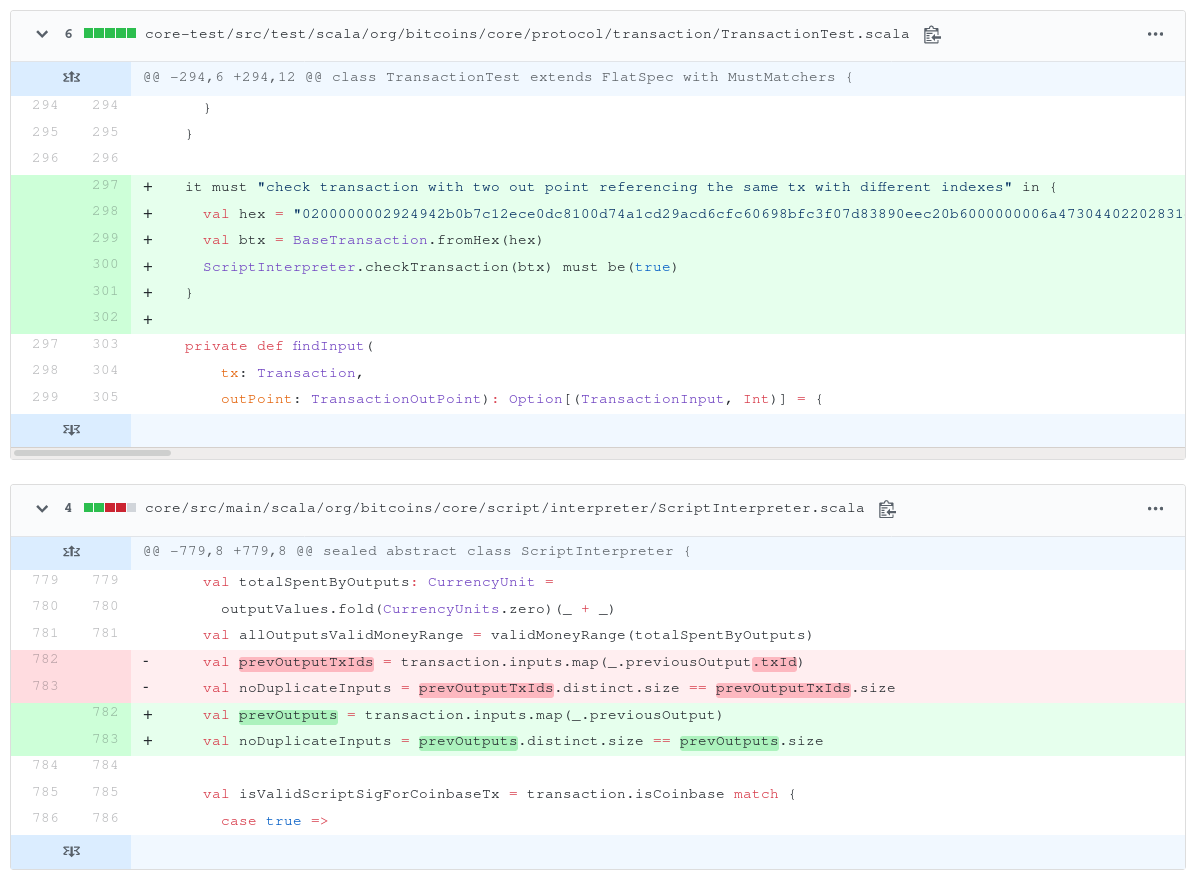
\includegraphics[width=\textwidth,height=0.8\textheight,keepaspectratio]{assets/bitcoin-s-pr.png}
\end{frame}


\end{document}
